\documentclass[twoside,twocolumn]{article}

\usepackage{blindtext}
\usepackage{graphicx}
\usepackage[sc]{mathpazo}
\usepackage[T1]{fontenc}
\linespread{1.05} 
\usepackage{microtype}


\usepackage[english]{babel}


\usepackage[hmarginratio=1:1,top=32mm,columnsep=20pt]{geometry}
\usepackage[hang, small,labelfont=bf,up,textfont=it,up]{caption}
\usepackage{booktabs}


\usepackage{lettrine}


\usepackage{enumitem}
\setlist[itemize]{noitemsep}


\usepackage{abstract}
\renewcommand{\abstractnamefont}{\normalfont\bfseries} 
\renewcommand{\abstracttextfont}{\normalfont\small\itshape} 


\usepackage{titlesec}
\renewcommand\thesection{\Roman{section}} % 
\renewcommand\thesubsubsection{\roman{subsubsection}} 
\titleformat{\section}[block]{\large\scshape\centering}{\thesection.}{1em}{}
\titleformat{\subsubsection}[block]{\large}{\thesubsubsection.}{1em}{}


\usepackage{fancyhdr} 
\pagestyle{fancy} % All pages have headers and footers
\fancyhead{} % Blank out the default header
\fancyfoot{} % Blank out the default footer
\fancyhead[L]{Comparativa de herramientas de Data StoryTelling} % Custom header text
\fancyhead[R]{April 2021} % Custom header text
\fancyfoot[RO,LE]{\thepage} % Custom footer text


\usepackage{titling}


\usepackage{hyperref}


%----------------------------------------------------------------------------------------
%	TILULOS
%----------------------------------------------------------------------------------------

\setlength{\droptitle}{-4\baselineskip}

\pretitle{\begin{center}\Huge\bfseries}
\posttitle{\end{center}} 
\title{Comparativa de herramientas de Data StoryTelling}
\author{Jose Arias, Jose Gutierrez, Posi Vargas, Rodrigo Yanqui, Roby Zuñiga}
\date{\today} 
\renewcommand{\maketitlehookd}{
\begin{abstract}
\noindent
    Data Storytelling o Storytelling basado en datos es una técnica que transforma la información disponible en una historia. Combina formatos de visualización de datos como gráficos, cuadros, mapas animados, entre otros con elementos narrativos. El objetivo es utilizar una cantidad de datos algo compleja para contar una historia de una manera simple y concisa.
\end{abstract}
\begin{abstract}
\noindent 
    Data Storytelling or Storytelling based on data is a technique that transforms the information available in a story. It combines data visualization formats such as graphics, tables, animated maps, among others with narrative elements. The objective is to use a somewhat complex amount of data to tell a story in a simple and concise way.
\end{abstract}
}

%----------------------------------------------------------------------------------------

\begin{document}

% Print the title
\maketitle

%----------------------------------------------------------------------------------------
%	INTRODUCCION
%----------------------------------------------------------------------------------------

\section{Introduccion}
\lettrine[nindent=0em,lines=3]{E}n una cultura cada vez más impulsada por la información, contar una historia a través de ella agrega credibilidad a cualquier estrategia de Marketing.\\[0.1in]
Otro beneficio de esta metodología es el alto grado de atracción de esos contenidos. Como veremos más adelante, estas historias cautivan a la audiencia, ayudando a mejorar las conversiones y la fidelidad con la marca.\\[0.1in]
Data Storytelling es una técnica que utiliza datos para contar una historia. Es una forma útil de presentar información, lo que significa que se puede utilizar tanto con audiencias internas como externas.\\[0.1in]
Sin embargo, es importante diferenciar la narración de datos de la visualización de datos. La visualización de datos consiste en representar datos de manera gráfica, no necesariamente contar una historia.\\[0.1in]
Si estás realizando la presentación de un informe, por ejemplo, puedes vender mejor una idea o explicar mejor un punto si utilizas gráficos, tablas o infografías, ya que dichos contenidos retienen la atención de tu audiencia de una manera que un texto o incluso un video no lo pueden hacer.\\[0.1in]
Facilitan el procesamiento de toda la información a la vez y la toma de decisiones.\\[0.1in]
El data storytelling va más allá de representar datos de una manera más atractiva. Consiste en mostrar cómo o por qué los datos cambiaron durante un período, y para eso es necesario reunir:
\begin{itemize}
    \item Una Narrativa
    \item Un Contexto
    \item Personajes
\end{itemize}

%----------------------------------------------------------------------------------------
%	DESARROLLO
%----------------------------------------------------------------------------------------

\section{Desarrollo}

\subsection{Data Storytelling}
Presentar los datos como una serie de tablas y gráficos desarticulados podría dar lugar a que el público tenga dificultades para comprenderlo, o peor aún, llegar a las conclusiones equivocadas, tergiversando dichos datos. Lo que puede conllevar a una toma de decisiones errónea y graves consecuencias para un determinado negocio.\\[0.1in]
Un ejemplo muy característico es el de comparar el trabajo de data storytelling con un iceberg, debido a que tiene mucho trabajo en su base, pero también tiene la parte más importante, la que verá el cliente, la empresa, es decir, nuestro público.\\[0.1in]
Un mal diseño o unas visualizaciones incorrectas pueden echar por tierra el resto del trabajo. Hay que tener un objetivo, impactar. Debemos ser capaces de transformar datos en historias que muestren las métricas clave, las comparaciones entre fechas y diagramas de dispersión, es decir, en mensajes persuasivos y efectivos que sean difíciles de olvidar.
\begin{center}
    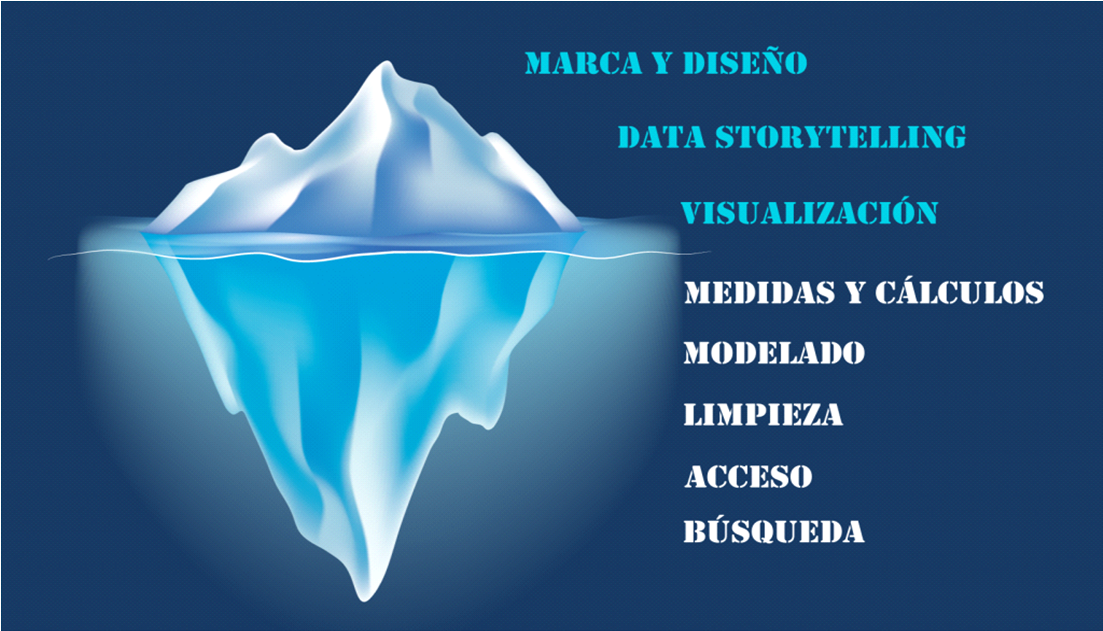
\includegraphics[width=7cm]{./img/img1.png}
\end{center}
Los humanos están programados para responder a las historias. Desde tiempos inmemorables, antes de que existiera la escritura, nuestros ancestros contaban historias para compartir información y experiencias con claros componentes didácticos y morales.\\[0.1in]
A una persona que se dedica a trabajar con datos le es fácil encontrar resultados en un informe, pero el resto de tu audiencia, ¿es capaz de entender lo que estás mostrando? Es por ello por lo que existe la necesidad de contar una historia para cerrar esa brecha y guiar al público a través de la lógica analítica.

\subsection{Factores}
Hoy en día debemos adaptar nuestras historias a los datos, y hemos de tener en cuenta numerosos factores:
\begin{itemize}
    \item Adaptar una historia a los datos, no al revés.
    \item Siempre debemos tratar con datos fiables.
    \item Hacer un buen uso de los datos, siempre respetando la privacidad de los individuos.
    \item Crear una narrativa que aporte valor.
    \item Utilizar una correcta visualización.
\end{itemize}

\subsection{Ventajas}
Lo más importante son las numerosas ventajas:
\begin{itemize}
    \item Identificar y actuar rápido sobre tendencias emergentes: hasta que los datos no son representados gráficamente es muy difícil identificar parámetros correlacionados;
    \item Comprensión ágil de la información: las gráficas permiten ver grandes volúmenes de datos de forma clara y coherente;
    \item Identificar relaciones y patrones dentro de los activos digitales: descubrir tendencias dentro de los datos permite una ventaja competitiva importante;
    \item Desarrollo de un nuevo lenguaje de negocio para contar la historia a terceros: gracias al storytelling es más fácil transmitir los mensajes a través de gráficos o visualizaciones elaboradas para lograr engagement.
\end{itemize}
En teoría, todo esto se ve realmente fácil de hacer, pero entonces, ¿por qué nos encontramos todos los días con pésimas presentaciones?\\[0.1in]
Existen varios programas de visualización de datos que permiten realizar numerosas visualizaciones avanzadas con las que sacar el máximo partido a los datos, como lo son Power BI, Tableau, Qlik, etcétera.
\begin{center}
    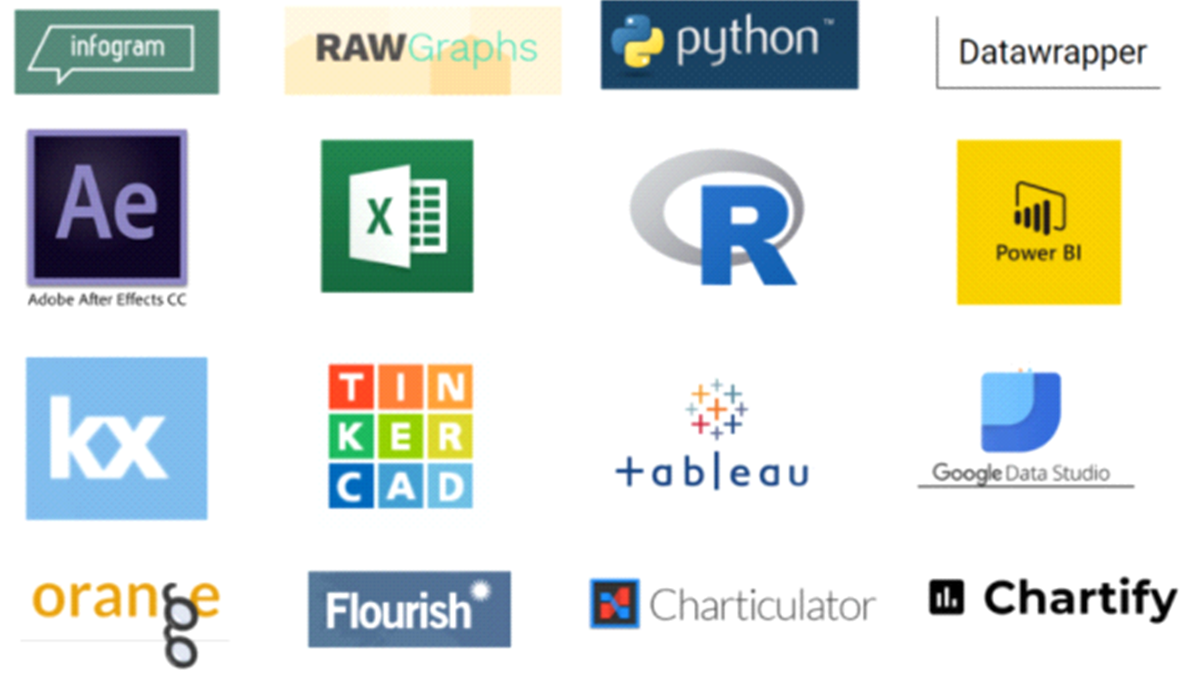
\includegraphics[width=7cm]{./img/img2.png}
\end{center}

\subsection{¿Porque es importante para una empresa?}
Algunas de las razones por las que es importante emplear esta herramienta dentro de una organización, o de manera personal, son las siguientes:
\begin{itemize}
    \item En primer lugar, la importancia radica en la riqueza de la información con la que se cuenta dentro de una base de datos y el aporte que esta brinda al momento de contar una historia.
    \item También permite simplificar toda la información que las organizaciones quieren transmitir a sus diferentes grupos de interés, ya sean clientes, colaboradores, proveedores, accionistas.
    \item Finalmente, permite representar de manera más sencilla y dinámica el mensaje. Empleando la narrativa, logramos que el mensaje sea interpretado de la manera en que deseamos.
\end{itemize}

\subsection{¿Que Empresas la Utilizan?}
\begin{itemize}
    \item \textbf{Airbnb}\\[0.1in]
    Story telling está en el corazón del marketing de Airbnb. Sus centros de mensajería se centran en la comunidad y la hospitalidad local, aprovechándolos deseos de los turistas para obtener más experiencias de viaje locales.\\[0.1in]
    Solo un ejemplo de cómo la marca utiliza los datos para contar historias atractivas, las historias de Airbnb resuenan constantemente con su público.\\
    \item \textbf{Spotify}\\[0.1in]
    Spotify recopila datos continuos sobre que canciones, listas de reproducción y artistas seleccionan sus 30 millones de usuarios.\\
    El servicio de transmisión de música combina esta información con los datos de ubicación y los datos demo gráficos de los oyentes, y la utiliza para crear contenido original para su blog Spotify Insights.\\[0.1in]
    El uso de los datos internos de esta manera ayuda a las marcas como Spotify a crear historias originales basadas en ideas a las que solo ellos pueden acceder, lo que les ayuda a diferenciarse de sus competidores.\\
    \item \textbf{Google}\\[0.1in]
    Los videos de "Año en la búsqueda" de Google se publican anualmente, utilizando sus datos para comunicar los términos más buscados, ofreciendo una perspectiva de "estado de la nación".\\[0.1in]
    Google logra evocar una gran variedad de emociones de los espectadores, aprovechando los eventos que han tocado a todos de alguna manera, utilizando datos para identificar exactamente que temas y eventos atraen a su audiencia.
\end{itemize}

\subsection{Herramientas de StoryTelling}
\paragraph{\Large Storify \\[0.1in]}
Storify es una de las herramientas más populares de storytelling. Con ella las historias en redes sociales tienen una fuerza especial: en Storify se puede integrar el contenido de diversas plataformas, como Twitter, Google+, Flickr o SoundCloud, en tu historia digital. El éxito de Storify comenzó con la documentación de eventos en vivo: ahora es una popular plataforma de blogs para narrar historias de todo tipo en tiempo real.\\[0.1in]
Esta herramienta también es una de las favoritas de los usuarios gracias a una interfaz sencilla e intuitiva. El contenido multimedia se arrastra y se coloca donde el usuario prefiera. Cuando la historia está terminada, se publica en la página web, en el blog o directamente en storify.com.\\[0.1in]
Storify también ayuda al usuario a estructurar dramatúrgicamente su relato digital ofreciendo elementos como titulares, cuerpo de texto y contenido multimedia para organizar la historia de forma efectiva. El texto dispuesto entre los archivos multimedia está limitado a 300 caracteres, un margen que puede sonar a limitación en un principio; sin embargo, este límite tiene sentido en cualquier historia digital: después de todo, las historias multimedia son atractivas precisamente por la brevedad y la precisión del contenido.\\

\noindent
\textbf{\large Ventajas:}
\begin{itemize}
    \item Ofrece integración con muchos medios sociales: Twitter, Facebook, Google+, App.net, YouTube, Flickr, Instagram, Chute, SoundCloud, Disqus, StockTwits, Tumblr y RSS.
    \item Los módulos de blogging en vivo son particularmente buenos.
    \item Versión básica gratuita.
\end{itemize}
\textbf{\large Desventajas:}
\begin{itemize}
    \item Para aplicaciones de pago: precio solo a demanda.
\end{itemize}
\textbf{\large Especialmente adecuado para:}
\begin{itemize}
    \item Profesionales que necesitan retransmitir eventos en tiempo real.
    \item Bloggers y periodistas.
\end{itemize}

\paragraph{\Large Shorthand \\[0.1in]}
Shorthand es una de las plataformas más utilizadas para la llamada scrollytelling. Esta herramienta proporciona un efecto visual especial al contenido. Se utiliza, por ejemplo, en informes de alta calidad, como los de la BBC o en campañas emocionales de diferentes ONG.\\[0.1in]
Uno de los sellos distintivos de esta herramienta de storytelling es la elevada calidad de las landing pages (páginas de destino) que se pueden crear para cada historia. El lector se desplaza por los capítulos, cada uno de los cuales se presenta en páginas diseñadas de forma individual. Para organizar el contenido multimedia se utiliza el clásico sistema de arrastrar y soltar. Se pueden integrar diferentes tipos de contenido: fotos, presentaciones de diapositivas, vídeos, mapas e infografías. Para que el lector tenga en todo momento el control de la experiencia del usuario, hay un menú en el que puede hacer clic para acceder a cada capítulo.\\[0.1in]
El registro en Shorthand es gratuito y la facturación tiene lugar por cada historia que se publica o con una suscripción anual. Al igual que otros tipos de software de storytelling, Shorthand sigue un modelo de costes individualizado: se realizan ofertas a petición de cada cliente potencial. Estos modelos de costes flexibles a veces pueden conllevar ventajas, pero también crean una falta de transparencia en una de las aplicaciones para contar historias más caras del mercado.\\

\noindent
\textbf{\large Ventajas:}
\begin{itemize}
    \item Diseño visual de las historias moderno y de gran calidad.
    \item Numerosos módulos y opciones de diseño.
\end{itemize}
\textbf{\large Desventajas:}
\begin{itemize}
    \item Sin derechos a un buen material de imagen no se puede sacar todo el potencial de la herramienta.
    \item Precios bastante altos en comparación con otras opciones del mercado.
\end{itemize}
\textbf{\large Especialmente adecuado para:}
\begin{itemize}
    \item Historias con material visual que debe impresionar a los lectores.
    \item Proyectos profesionales con un gran presupuesto.
\end{itemize}

\subsection{COMPARATIVA STORIFY VS SHORTHAND}
\begin{center}
    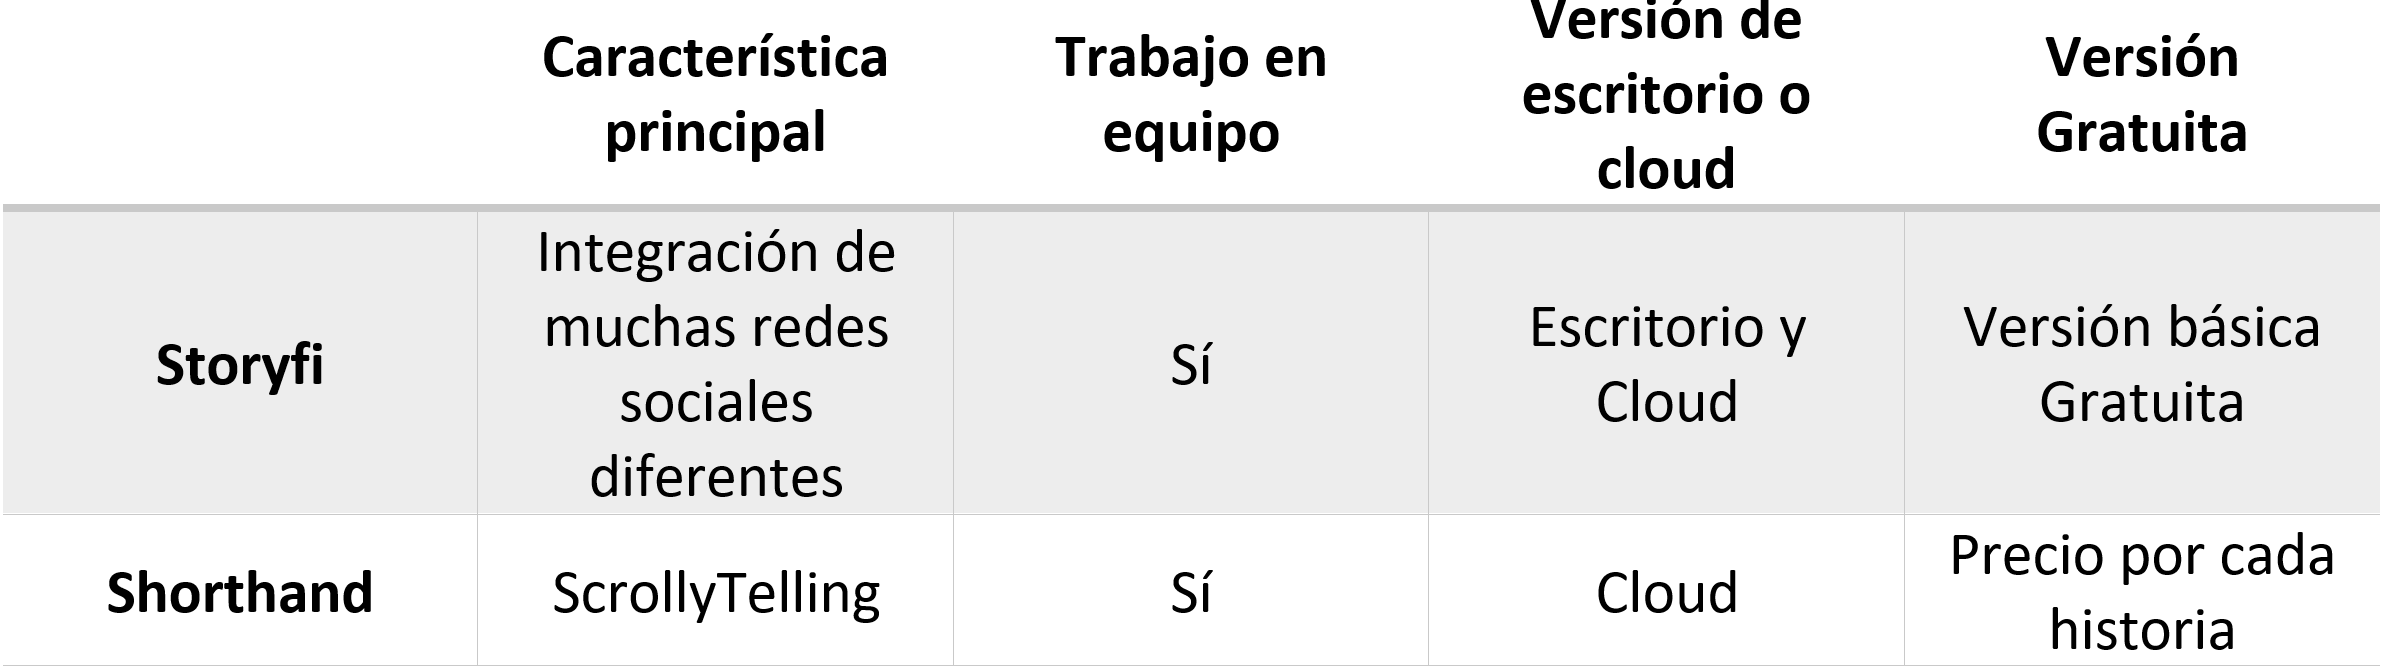
\includegraphics[width=7cm]{./img/img3.png}
\end{center}

%----------------------------------------------------------------------------------------
%	CONCLUSIONES
%----------------------------------------------------------------------------------------

\section{Conclusiones}
En conclusión, el Data Storytelling empleado de manera correcta, mejorara la comunicación entre grupos dentro de una organización, ya que se lograría transmitir las metas y objetivos claros; pero adicionalmente, es importante contar con las personas con las habilidades de comunicación indicadas y poder interpretar los datos encontrados.\\[0.1in]
Esta es una habilidad que debemos desarrollar todos nosotros ya que en el futuro será un requisito mínimo requerido por todas las empresas que bus-can candidatos potenciales para formar parte de equipo de colaboradores.\\[0.1in]
Los datos son útiles, solo si somos capaces de:
\begin{itemize}	
    \item Acceder a ellos
    \item Entenderlos
    \item Tomar medidas al respecto
\end{itemize}
Y reconoceremos una buena visualización de datos cuando… Seamos capaces de entender qué transmite en pocos segundos.\\[0.1in]
Las grandes historias no son aquellas que duran mucho, sino que logran decir mucho en poco espacio. Para conseguir un buen storytelling hay que ir a lo importante, tanto para la audiencia como para la propia empresa.

%----------------------------------------------------------------------------------------
%	RECOMENDACIONES
%----------------------------------------------------------------------------------------

\section{Recomendaciones}
Hay que tener en cuenta que se quiere contar, a quien se quiere contar y como se organizara la información para transmitir este mensaje.

%----------------------------------------------------------------------------------------
%	BIBLIOGRAFIA
%----------------------------------------------------------------------------------------

\begin{thebibliography}{99} 
    \bibitem{}
    Walsh, A. (2020). What is Data Storytelling? Recuperado de 
    \\\texttt{https://cutt.ly/bvE5RQq}
    \bibitem{}
    Galiana, P. (2019). LData Storytelling, qué es y cómo puede mejorar tu estrategia de contenidos. Recuperado de 
    \\\texttt{https://cutt.ly/svE5n2C}
    \bibitem{}
    Dykes, B. (s.f.). Data Storytelling: The Essential Data Science Skill Everyone Needs. Recuperado de 
    \\\texttt{https://cutt.ly/JvE5lRd}
    \bibitem{}
    Puro Marketing. (2018). 6 consejos para mejorar los resultados del storytelling. Recuperado de 
    \\\texttt{https://cutt.ly/BvE5g1s}
    \bibitem{}
    Ionos. (2018). Herramientas de storytelling: cómo funciona la narrativa digital. Recuperado de 
    \\\texttt{https://cutt.ly/BvE5g1s}
\end{thebibliography}
%----------------------------------------------------------------------------------------
\end{document}